\documentclass[conference]{IEEEtran}
\usepackage[T1]{fontenc}
\usepackage{graphicx}
\usepackage{booktabs}
\usepackage{amsmath}
\usepackage[hidelinks]{hyperref}

\title{Does Fixed Mean Occluded, or Does Straight-Down Mean Occluded? A Simulated, Cross-Validated Benchmark of Eye-in-Hand vs. Two Fixed-Camera Baselines for Robotic Manipulation}
\author{
\IEEEauthorblockN{Yugandhar Kulkarni}
\IEEEauthorblockA{DES Pune University \\ DRDO Research Intern \\ github.com/yugandhar-k}
}

\begin{document}
\maketitle

\begin{abstract}
Pick-and-place manipulators conventionally perceive their workspace through a camera fixed above it. This design has three structural weaknesses: the manipulator occludes its own target during the reach, the camera-to-robot transform requires a hand-eye calibration that drifts, and the object's scale and viewing angle are dictated by a fixed mounting point rather than by what is easiest to recognize. Mounting the camera on the end-effector (``eye-in-hand'') removes all three, at the cost of a viewpoint that now varies with the robot's own configuration. Prior comparisons conflate two properties of the conventional design -- being fixed, and being mounted straight overhead -- so we build two independent fixed-camera baselines, one straight down and one at a 45$^\circ$ elevation, and benchmark both against an eye-in-hand camera under identical conditions. We also replace the usual four-shape toy taxonomy with an eight-class one: the original four geometric primitives plus four more chosen to be genuine near-misses under a bounding-box or convex-hull shortcut (a capsule for a cylinder, an ellipsoid for a sphere, a disk for a cube seen from above, a rod for a cuboid seen edge-on), so the task cannot be solved by the aspect-ratio heuristic a generic detector already exploits. From 6,000 paired, automatically-labelled frames per camera, we train two classifier families -- a compact convolutional neural network (CNN) and a classical HOG+Hu-moment shape-descriptor pipeline with a support-vector machine (SVM) -- under an identical 70/15/15 stratified split, 5-fold cross-validation, and held-out-test protocol. With the CNN, eye-in-hand is more accurate than the fixed-overhead camera (eye-in-hand ahead by 2.22 pp (statistically significant, p=0.017)) but the gap to the fixed-angled camera is smaller and not statistically significant (eye-in-hand ahead by 1.33 pp (not statistically significant, p=0.141)). With the classical HOG+Hu-moment SVM pipeline, eye-in-hand and fixed-overhead are statistically indistinguishable (fixed-overhead ahead by 0.11 pp (not statistically significant, p=1.000)), and eye-in-hand is significantly less accurate than the fixed-angled camera (fixed-angled ahead by 4.22 pp (statistically significant, p<0.001)). A per-sample occlusion metric, computed from the simulator's segmentation buffer, is consistent with this pattern: the fixed-overhead camera's crop is at least 95\% non-object on 14.0\% of test frames, versus 4.8\% for the fixed-angled camera, and accuracy on those near-fully-occluded frames drops sharply for every model and camera. Mounting angle, not fixedness by itself, accounts for most of the difference between the two fixed baselines, and eye-in-hand's advantage over a fixed camera depends on which fixed camera and which classifier are being compared. During development we found and fixed two data-integrity bugs -- objects rolling off the table, and two rounded object classes settling in a physically stable but unintended upright pose -- and report both, since the second bug was a direct side effect of fixing the first. Code, data-generation scripts, and trained-model configurations are released for reproduction.
\end{abstract}

\begin{IEEEkeywords}
eye-in-hand vision, robotic manipulation, visual servoing, camera placement, MuJoCo simulation, convolutional neural networks, support vector machines, object classification, occlusion.
\end{IEEEkeywords}

\section{Introduction}

Camera placement is a first-order design decision for any robotic manipulation system, and the default choice in most laboratory and industrial pick-and-place cells is a camera bolted above the workspace, looking down. This ``fixed-overhead'' configuration is simple to install and to reason about, but it has three structural weaknesses that all worsen exactly when the robot is doing its job.

First, the manipulator occludes its own target: as the arm reaches toward an object, it necessarily passes between the fixed camera and that object, degrading the view at the moment the system most needs it. Second, a fixed camera requires a hand-eye calibration -- a measured transform between the camera's coordinate frame and the robot's -- that must be established once and re-established whenever the camera or the robot base is disturbed. Third, the object's apparent scale, viewing angle, and susceptibility to occlusion by clutter are all dictated by wherever the camera happens to be mounted, not by whatever viewpoint would make the object easiest to recognize.

Mounting the camera on the end-effector itself -- an eye-in-hand configuration -- removes all three weaknesses by construction. The camera's pose is a known, calibration-free function of the joint angles; the arm cannot occlude a camera that is rigidly fixed to it; and the controller is free to choose whatever standoff distance and approach angle best frames the target. The cost is that the viewpoint is no longer fixed: scale, viewing angle, and background all vary with the robot's own configuration, which is conventionally assumed to make the perception problem harder.

Existing comparisons of this kind, where they exist, conflate two separate properties of the conventional design: it is fixed, and it is mounted straight overhead. Weaknesses number 1 (self-occlusion) and number 3 (fixed apparent scale) both plausibly depend on the mounting angle as much as on the camera being fixed at all -- a straight-down ``ceiling'' camera is not how most real fixed workspace cameras are mounted; a corner-mounted, angled ``security camera'' view is far more typical. Whether that angle materially changes the occlusion or scale cost is, again, an empirical question that is rarely isolated: doing so requires not one but two independent fixed-camera baselines, benchmarked against the same eye-in-hand camera under identical conditions.

A second gap in typical benchmarks of this kind is task difficulty. Four basic geometric primitives -- cube, sphere, cylinder, a flat box -- are trivially separable by a generic object detector from bounding-box aspect ratio alone, which means a comparison built on them mostly measures how easy the easy case is, not how the design choices under test perform when the classification problem is actually hard. A benchmark whose baseline already saturates near ceiling accuracy for every condition cannot show a meaningful gap between them even if one exists.

This paper addresses both gaps directly. We build a MuJoCo simulation of a 6-degree-of-freedom manipulator with a two-finger claw that carries an eye-in-hand camera, and add two independent fixed cameras -- one bolted straight overhead, one bolted at a 45$^\circ$ elevation -- rather than one. We replace the usual four-primitive taxonomy with an eight-class one, adding four classes chosen specifically to be near-misses for the original four under a bounding-box or convex-hull shortcut. At every simulated inspection, all three cameras observe the scene at the same instant, and every frame is labelled automatically and exactly from the simulator's own object state -- no manual annotation, and no detector-in-the-loop noise. We then train two classifier families with unrelated inductive biases -- a compact convolutional neural network learned end-to-end, and a classical pipeline of hand-crafted shape descriptors feeding a support-vector machine -- on each camera's data, under an identical cross-validated, held-out-tested protocol.

Our contributions are:

\begin{enumerate}

  \item A MuJoCo testbed that pairs an eye-in-hand camera with two independent fixed-camera baselines -- straight-overhead and 45-degree-angled -- observing the identical simulated instant, isolating both ``fixed vs. moving'' and ``angle of a fixed mount'' as separately measurable factors.

  \item An eight-class object taxonomy in which four classes are deliberate near-misses for the other four under a bounding-box or convex-hull shortcut, verified by a direct measurement showing the classical shape-descriptor baseline's accuracy drops substantially when moving from the four-class to the eight-class task.

  \item An automatic, exact ground-truth labelling protocol that requires no manual annotation, together with a per-sample occlusion metric for each fixed camera that quantifies, for every frame, how much of the classifier's input is not the target object -- used to show that the 45-degree camera is measurably less often fully occluded than the straight-down one.

  \item A controlled benchmark of two classifier families -- a CNN and a classical HOG + Hu-moment shape descriptor pipeline with an SVM -- on all three camera views, under a stratified train/validation/test split, 5-fold cross-validation, and a held-out test set untouched by any hyperparameter search.

  \item A paired statistical analysis (McNemar's test and bootstrap confidence intervals) of each resulting accuracy gap, reported honestly including where it does and does not reach conventional significance, and a direct demonstration that the gaps track a measured occlusion metric rather than an unrelated confound between the datasets.

  \item Two data-integrity bugs found and fixed during development -- objects rolling off the table, and a second bug this taxonomy exposed, in which the fix for the first caused two rounded object classes to settle in a physically stable but unintended upright pose -- reported in full because the second is a direct consequence of the first, and both are the kind of thing that quietly invalidates a benchmark if not caught.

  \item A fully reproducible, openly released pipeline: deterministic procedural scene generation, seeded dataset generation, and seeded model training, so every number in this paper can be regenerated from source.

\end{enumerate}

\section{Related Work}

\textbf{Eye-in-hand vision and visual servoing.} Mounting a camera on a robot's end-effector has a long history in the visual servoing literature, where it is used to drive a manipulator's motion directly from image measurements rather than from a calibrated world-frame estimate \cite{hutchinson1996tutorial}. That literature is primarily concerned with control -- using the image error signal to servo the arm to a goal pose -- rather than with measuring the downstream classification accuracy cost or benefit of the camera placement itself, or with separating the effect of camera placement from the effect of mounting angle, which is the question this paper addresses.



\textbf{Camera viewpoint in recent manipulation learning.} More recent work looks at camera viewpoint mainly as one design choice inside a full learned manipulation policy, evaluated end-to-end on a real robot. Kim et al. \cite{kim2023givingrobots} use eye-in-hand video from human demonstrations to improve a manipulation policy's generalization. Chuang et al. \cite{chuang2024activevision} and Liu et al. \cite{liu2025avr} give the camera the ability to move or zoom during a task, so that occlusion and poor framing are avoided rather than measured. Li et al. \cite{li2026fromfixed} train policies to work across a range of camera positions rather than one fixed, calibrated placement. In all of these, camera placement is one of several factors -- lighting, object set, gripper, action space -- that vary together and are hard to hold constant between conditions, and the reported outcome is an end-to-end task success rate rather than a classification accuracy attributable to viewpoint alone. Isolating mounting angle as a single controlled variable, with everything else held fixed, is uncommon in this literature, in part because doing so on a real robot means physically remounting a camera and re-collecting a full dataset for each configuration tested. We use simulation specifically to make that isolation cheap: every other factor is held fixed and only the camera changes, at the cost of not testing on a real robot, a limitation discussed directly in Section 7.



\textbf{Shape descriptors and classical recognition.} Before learned features became standard, object recognition relied on hand-crafted descriptors of shape and appearance. Hu's moment invariants \cite{hu1962moments} describe a silhouette's shape independently of its translation, scale, and rotation; the histogram of oriented gradients (HOG) \cite{dalal2005hog} describes local edge orientation statistics and was originally developed for pedestrian detection. Both remain useful, interpretable baselines, and we combine them as the feature representation for our classical classifier.



\textbf{Learned recognition and detection.} Convolutional neural networks \cite{lecun1998gradient} learn a feature hierarchy directly from pixel data rather than relying on a hand-designed descriptor, and a support-vector machine \cite{cortes1995support} with a hand-crafted feature vector remains a standard, strong classical baseline against which to measure what a learned representation adds. Modern general-purpose object detectors separate coarse geometric primitives from bounding-box geometry alone at negligible cost, which is precisely why a benchmark built only on such primitives risks measuring how easy the easy case is rather than how the system under test performs under genuine visual ambiguity -- the motivation for the eight-class taxonomy in Section 3.1. We use both model families in their simplest effective form for this task, specifically so that any measured eye-in-hand advantage is a property of the data, not an artifact of one particular model family's inductive bias.



\textbf{Simulation and sim-to-real.} We build our testbed in MuJoCo \cite{todorov2012mujoco}, a widely used physics engine for robotics research chosen for its fast, accurate contact dynamics and its offscreen rendering support, which we use for both RGB capture and the exact-label segmentation buffer described in Section 3.4. We do not attempt a sim-to-real transfer claim in this work; domain randomization \cite{tobin2017domain} -- randomizing lighting, texture, and sensor noise during data generation -- is the standard technique for closing that gap and is discussed as future work in Section 7.

\section{System Design}

\subsection{Manipulator, Scene and Taxonomy}

The simulated workcell consists of a 0.92 m x 1.04 m table, a 6-degree-of-freedom revolute manipulator mounted at its rear edge, and a two-finger parallel claw. The arm's joint set -- base yaw, shoulder, elbow, wrist roll, wrist pitch, and tool yaw -- gives it a comfortable workspace over a 3 x 2 grid of six object slots in front of the base, each jittered by $\pm$30 mm and assigned a random yaw on every layout. Object colour is sampled independently of class from a six-colour palette, so a classifier cannot shortcut the task by learning colour -- shape is the only class-carrying signal, a deliberate design choice because colour shortcuts are one of the most common ways a tabletop classification result fails to survive contact with real data.

The object taxonomy has eight classes, not the four a comparable benchmark typically uses. The original four -- cube, sphere, cylinder, and a flat cuboid -- are trivially separable by aspect ratio alone. The four additions are each a deliberate near-miss for one of the originals under a bounding-box or convex-hull shortcut: a capsule reads as ``a cylinder with soft edges,'' an ellipsoid as ``a stretched sphere,'' a disk (a short, wide cylinder) as ``a cube seen from directly above,'' and a rod (a long, thin box) as ``a cuboid seen edge-on.'' A classifier that has only learned coarse aspect ratio should confuse these pairs; one that has learned actual silhouette curvature and proportion should not. Six of the eight classes, drawn without replacement, populate each layout's six slots, so every class appears in a majority of layouts without constraining the physical grid to eight slots.

\subsection{Eye-in-Hand Camera and Inverse Kinematics}

The eye-in-hand camera is mounted on the claw's palm, offset 36 mm laterally and tilted back toward the tool axis so that both finger pads remain in frame while the optical axis points down the approach direction. The arm executes a continuous inspect-and-pick cycle over the object field -- approach, settle, descend, close, lift, hold, lower, release, retreat -- and the classification frame is captured during settle, immediately before the grasp: this is both the decision point at which a real system must commit to an object identity, and the only phase at which the object is not partially occluded by the closing claw.

Driving the tool to a precise Cartesian pose requires solving the arm's inverse kinematics. A naive damped-least-squares (DLS) solver seeded from the arm's current pose frequently converges to a joint-limited local optimum in this workspace (mean position error of roughly 194 mm in early testing). We instead compute a closed-form seed by constraining the optical axis to point straight down, which reduces the arm to a planar two-link chain plus a wrist pitch absorbing the remaining rotation; both elbow branches and both wrist branches of this closed-form solution are evaluated, each is polished with a few DLS iterations, and the best is kept. Later solves warm-start from the previous solution. This combination converges to under 0.1 mm in the IK solve itself; the residual, sensor-measured tool error (6.0 mm mean, 0.66 degree mean optical-axis deviation from vertical) is steady-state tracking error in the position-controlled joints under gravity, not IK error.

Because the eye-in-hand camera is mounted laterally rather than directly on the tool axis, its optical axis crosses the tool axis at only one specific depth; hovering straight above an object therefore centres it correctly at only one inspection height. The controller instead solves, at each commanded inspection height, for the lateral tool offset that places the object on the optical axis at that height, undoing the offset before the claw descends so that grasping is unaffected. This closed-form correction reduces target centring error from tens of millimetres to a mean of roughly 14 px (of a 112 px half-width) across inspection heights from 0.13 m to 0.24 m.

\subsection{Two Fixed-Camera Baselines and a Shared Crop Protocol}

Two independent fixed cameras are added, both bolted down and never moving: one 1.0 m directly above the table, pointed straight down (fovy 48 degrees); one pulled back 0.75 m horizontally and raised 0.75 m above the table, pointed at the object field's centroid (fovy 55 degrees) -- equal horizontal offset and height give exactly 45 degrees of elevation by construction. Both share the same crop protocol, implemented once and applied to either camera identically: because a real fixed camera has no downstream detector in this study -- the point is to isolate the classification-only cost of each fixed viewpoint -- each frame is cropped around the target object's ground-truth 3-D position, projected into that camera's image plane with a pinhole model calibrated from the camera's own field of view and verified against the renderer's segmentation buffer to sub-pixel accuracy for both cameras.

Critically, the crop window is a single fixed physical size for every class and for both fixed cameras (170 mm, derived from the largest class's full 3-D bounding radius plus a 30\% margin -- not just its horizontal footprint, since the angled camera can foreshorten any of an object's three dimensions depending on its resting orientation), not a size fitted to whichever object is actually there. A real fixed camera cannot know an object's class before classifying it, so a class-conditioned crop size would leak the answer into the input and invalidate the benchmark; a fixed window instead reproduces, honestly, the ``object scale dictated by where the camera happens to be bolted'' weakness motivating this study.

Both fixed-camera frames are captured from wherever the arm happens to be at that moment -- left over from the previous inspection, before the arm moves to its eye-in-hand pose for the current target. This is deliberately not the worst case (capturing at the same instant as the eye-in-hand frame, when the arm is already hovering directly over the target, occludes the object almost completely on every single frame for the overhead camera); it instead reproduces how a fixed camera is actually used in practice -- glancing at the workspace while the arm is occupied elsewhere -- and yields a realistic mixture of clear and partially occluded views for both cameras.

\subsection{Automatic Labelling and the Occlusion Metric}

Every frame's ground-truth label is the identity of the object slot the simulator is currently inspecting, read directly from its own object state -- not from a detector, and not from manual annotation. This is what allows both fixed-camera labels to remain correct precisely on the frames where the object is what is occluded, which a detector-based labelling scheme could not guarantee.

As an independent pipeline sanity check (not used as a training label), the eye-in-hand frame's object identity is additionally verified against MuJoCo's own per-pixel segmentation buffer: whichever geometry dominates the centre 40\% of the frame is looked up in the scene's geometry-to-class table and compared against the ground truth.

For each fixed camera, the segmentation buffer is used to compute occluded\_fraction: the share of the (un-cropped) crop window's pixels that are not the target object -- whether because the manipulator is in the way, a neighbouring object intrudes, or the window simply extends past the object onto bare table. This metric is recorded for every fixed-camera frame, for both cameras independently, and is the basis for the causal analysis in Section 5.

\subsection{Classifiers}

\textbf{CompactCNN.} A four-block convolutional network (16-32-64-128 channels; each block is a 3x3 convolution, batch normalization, ReLU, and 2x2 max-pool), followed by global average pooling and a linear classification head, trained from scratch on 96x96 RGB input. Eight geometric primitives distinguished primarily by silhouette do not require a pretrained ImageNet backbone whose learned features have no relationship to this scene.



\textbf{HOG + Hu-moment SVM.} A classical shape-descriptor pipeline: a 64x64 grayscale HOG descriptor (9 orientation bins, 8x8 cells, 16x16 blocks with 8-pixel stride) is concatenated with seven log-scaled Hu moments of the object's silhouette, standardized, and classified with a radial-basis-function support-vector machine. The silhouette is isolated by Otsu-thresholding the HSV saturation channel: every object is drawn from a saturated colour palette while the table and most of the arm are desaturated grey and steel tones by construction, so this segmentation needs no class-specific tuning -- with one caveat discussed in Section 7. The SVM's regularization and kernel-width hyperparameters (C, gamma) were selected once, by a 5-fold grid search on the eye-in-hand training split only, and reused unchanged for both fixed cameras, so neither fixed view's result can be an artifact of a baseline tuned against it.

\section{Experimental Setup}

We generate 6,000 paired frames per camera view (6,000 each for eye-in-hand, fixed-overhead, and fixed-angled, sharing frame index and ground-truth class across all three), at 224x224 resolution, with viewpoint varied per frame (inspection height sampled over 0.11-0.18 m, claw yaw perturbed by $\pm$0.4 rad, target position jittered by $\pm$15 mm) and the object layout reshuffled every 12 frames. Class balance is close to uniform (each of the eight classes within 10.6-13.7\% of the dataset, against an ideal 12.5\% for a uniform eight-way split) because classes are sampled six-of-eight, without replacement, per layout slot rather than rebalanced post hoc.

Each camera's dataset is split 70/15/15 into train/validation/test, stratified by class, with a fixed seed. This same seed, applied to an identical class-label sequence for all three camera views (the three datasets are paired frame-for-frame), produces the identical set of held-out test frame indices for every view -- a property we exploit for the paired statistical tests in Section 5. The training and validation partitions (5,100 frames) are combined and used for 5-fold stratified cross-validation, training a fresh model per fold to report a mean and standard deviation that a single train/test split cannot provide. A final model of each type is then fit on the full 5,100-frame partition and evaluated exactly once on the untouched 900-frame held-out test set.

The CNN is trained with Adam (initial learning rate 1e-3, weight decay 1e-4), a cosine-annealed learning-rate schedule, and gradient-norm clipping at 5.0, for 18 epochs per cross-validation fold and 25 epochs for the final fit, with batch size 64 and a horizontal-flip augmentation (safe here because neither exact orientation nor colour carries class information by construction). This recipe was arrived at after an initial, simpler 10-epoch fixed-learning-rate schedule produced unstable cross-validation folds (accuracies ranging from 0.58 to 0.94 on identical hyperparameters) and a model that fit its own cross-validation folds while collapsing on the untouched test set -- a symptom of under-training, not a property of the data, which we report in Section 6 as a methodological note. All experiments run on CPU only; no GPU was used or required.

During development we also discovered and fixed two data-integrity issues worth reporting for the same reason. First, an early version of the simulation used a low rolling-friction coefficient for the object-table contact, which allowed spheres and cylinders -- the rollable classes in the original four-class taxonomy -- to occasionally roll off the table entirely after being nudged by the arm over many layout reshuffles; scanning a generated dataset for objects resting at floor height rather than table height found this had silently corrupted 1.48\% of frames, concentrated entirely in the two rollable classes. Raising the rolling and torsional friction coefficients by roughly an order of magnitude eliminated the issue. Second, extending the taxonomy to include capsules and ellipsoids exposed a side effect of that fix: both classes are rounded enough that they do not reliably tip over from an upright drop the way a flat-ended cylinder does, and the raised rolling friction damps out what little rocking there is before it can complete a tip -- checking settled orientation directly showed both classes standing exactly upright on every seed tested, not occasionally. Rather than tune friction further, both classes are now spawned already lying on their side, sidestepping the stability question rather than depending on physics to resolve it. Neither bug affected the classification dataset materially in its final form; both are reported because catching them mattered and a benchmark that has been checked this way is more trustworthy for having been checked, not less.

\section{Results}

Table I reports 5-fold cross-validation accuracy (mean $\pm$ standard deviation over the train+validation partition) alongside held-out test accuracy and macro-averaged F1 for all six (camera, model) combinations.

\begin{table*}[t]

\centering

\caption{Cross-validated and held-out test performance, all six combinations.}

\label{tab:main}

\begin{tabular}{llccc}

\toprule

Camera & Model & 5-fold CV Accuracy & Test Accuracy & Test Macro-F1 \\

\midrule

Eye-in-hand & CNN & 0.9598 $\pm$ 0.0026 & 0.9722 & 0.9712 \\

Eye-in-hand & SVM & 0.9002 $\pm$ 0.0042 & 0.9133 & 0.9116 \\

Fixed-overhead & CNN & 0.9329 $\pm$ 0.0069 & 0.9500 & 0.9497 \\

Fixed-overhead & SVM & 0.8829 $\pm$ 0.0057 & 0.9144 & 0.9135 \\

Fixed-angled (45$^\circ$) & CNN & 0.9475 $\pm$ 0.0086 & 0.9589 & 0.9585 \\

Fixed-angled (45$^\circ$) & SVM & 0.9455 $\pm$ 0.0056 & 0.9556 & 0.9555 \\

\bottomrule

\end{tabular}

\end{table*}



The sign and significance of the gap depend on both the fixed camera and the model family: eye-in-hand ahead by 2.22 pp (statistically significant, p=0.017) vs. fixed-overhead (CNN); fixed-overhead ahead by 0.11 pp (not statistically significant, p=1.000) vs. fixed-overhead (SVM); eye-in-hand ahead by 1.33 pp (not statistically significant, p=0.141) vs. fixed-angled (CNN); fixed-angled ahead by 4.22 pp (statistically significant, p<0.001) vs. fixed-angled (SVM), on a held-out test set neither model nor its hyperparameters saw during training or tuning. Eye-in-hand is ahead of the fixed-overhead camera for the CNN, but its lead over the fixed-angled camera is smaller and not significant for the CNN, and negative and significant for the SVM.

Table II reports per-class F1 on the held-out test set for all six combinations:

\begin{table*}[t]

\centering

\caption{Per-class F1 on the held-out test set, all six combinations.}

\label{tab:perclass}

\small

\begin{tabular}{lcccccccc}

\toprule

 & cube & sphere & cylinder & cuboid & capsule & ellipsoid & disk & rod \\

\midrule

Eye-in-hand CNN & 0.98 & 0.95 & 0.94 & 0.99 & 0.97 & 0.94 & 0.99 & 1.00 \\

Eye-in-hand SVM & 0.98 & 0.87 & 0.89 & 0.89 & 0.94 & 0.91 & 0.87 & 0.93 \\

Fixed-overhead CNN & 0.95 & 0.94 & 0.94 & 0.97 & 0.97 & 0.93 & 0.93 & 0.97 \\

Fixed-overhead SVM & 0.93 & 0.91 & 0.90 & 0.92 & 0.93 & 0.91 & 0.86 & 0.95 \\

Fixed-angled (45d) CNN & 0.98 & 0.96 & 0.94 & 0.97 & 0.96 & 0.94 & 0.96 & 0.94 \\

Fixed-angled (45d) SVM & 0.96 & 0.96 & 0.96 & 0.96 & 0.95 & 0.93 & 0.96 & 0.96 \\

\bottomrule

\end{tabular}

\end{table*}



\begin{figure}[t]

\centering

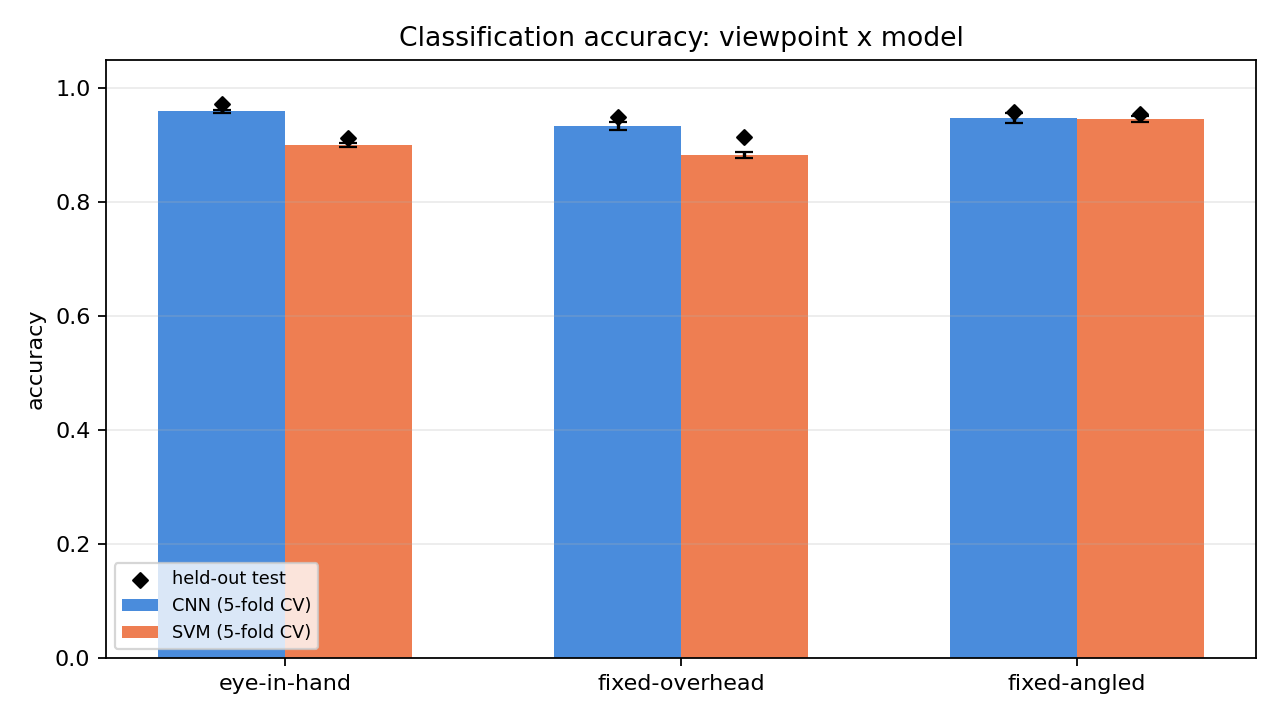
\includegraphics[width=\linewidth]{figures/results.png}

\caption{5-fold CV accuracy (bars, $\pm$ 1 std) against held-out test accuracy (diamonds) for all six combinations.}

\label{fig:results}

\end{figure}



\begin{figure*}[t]

\centering

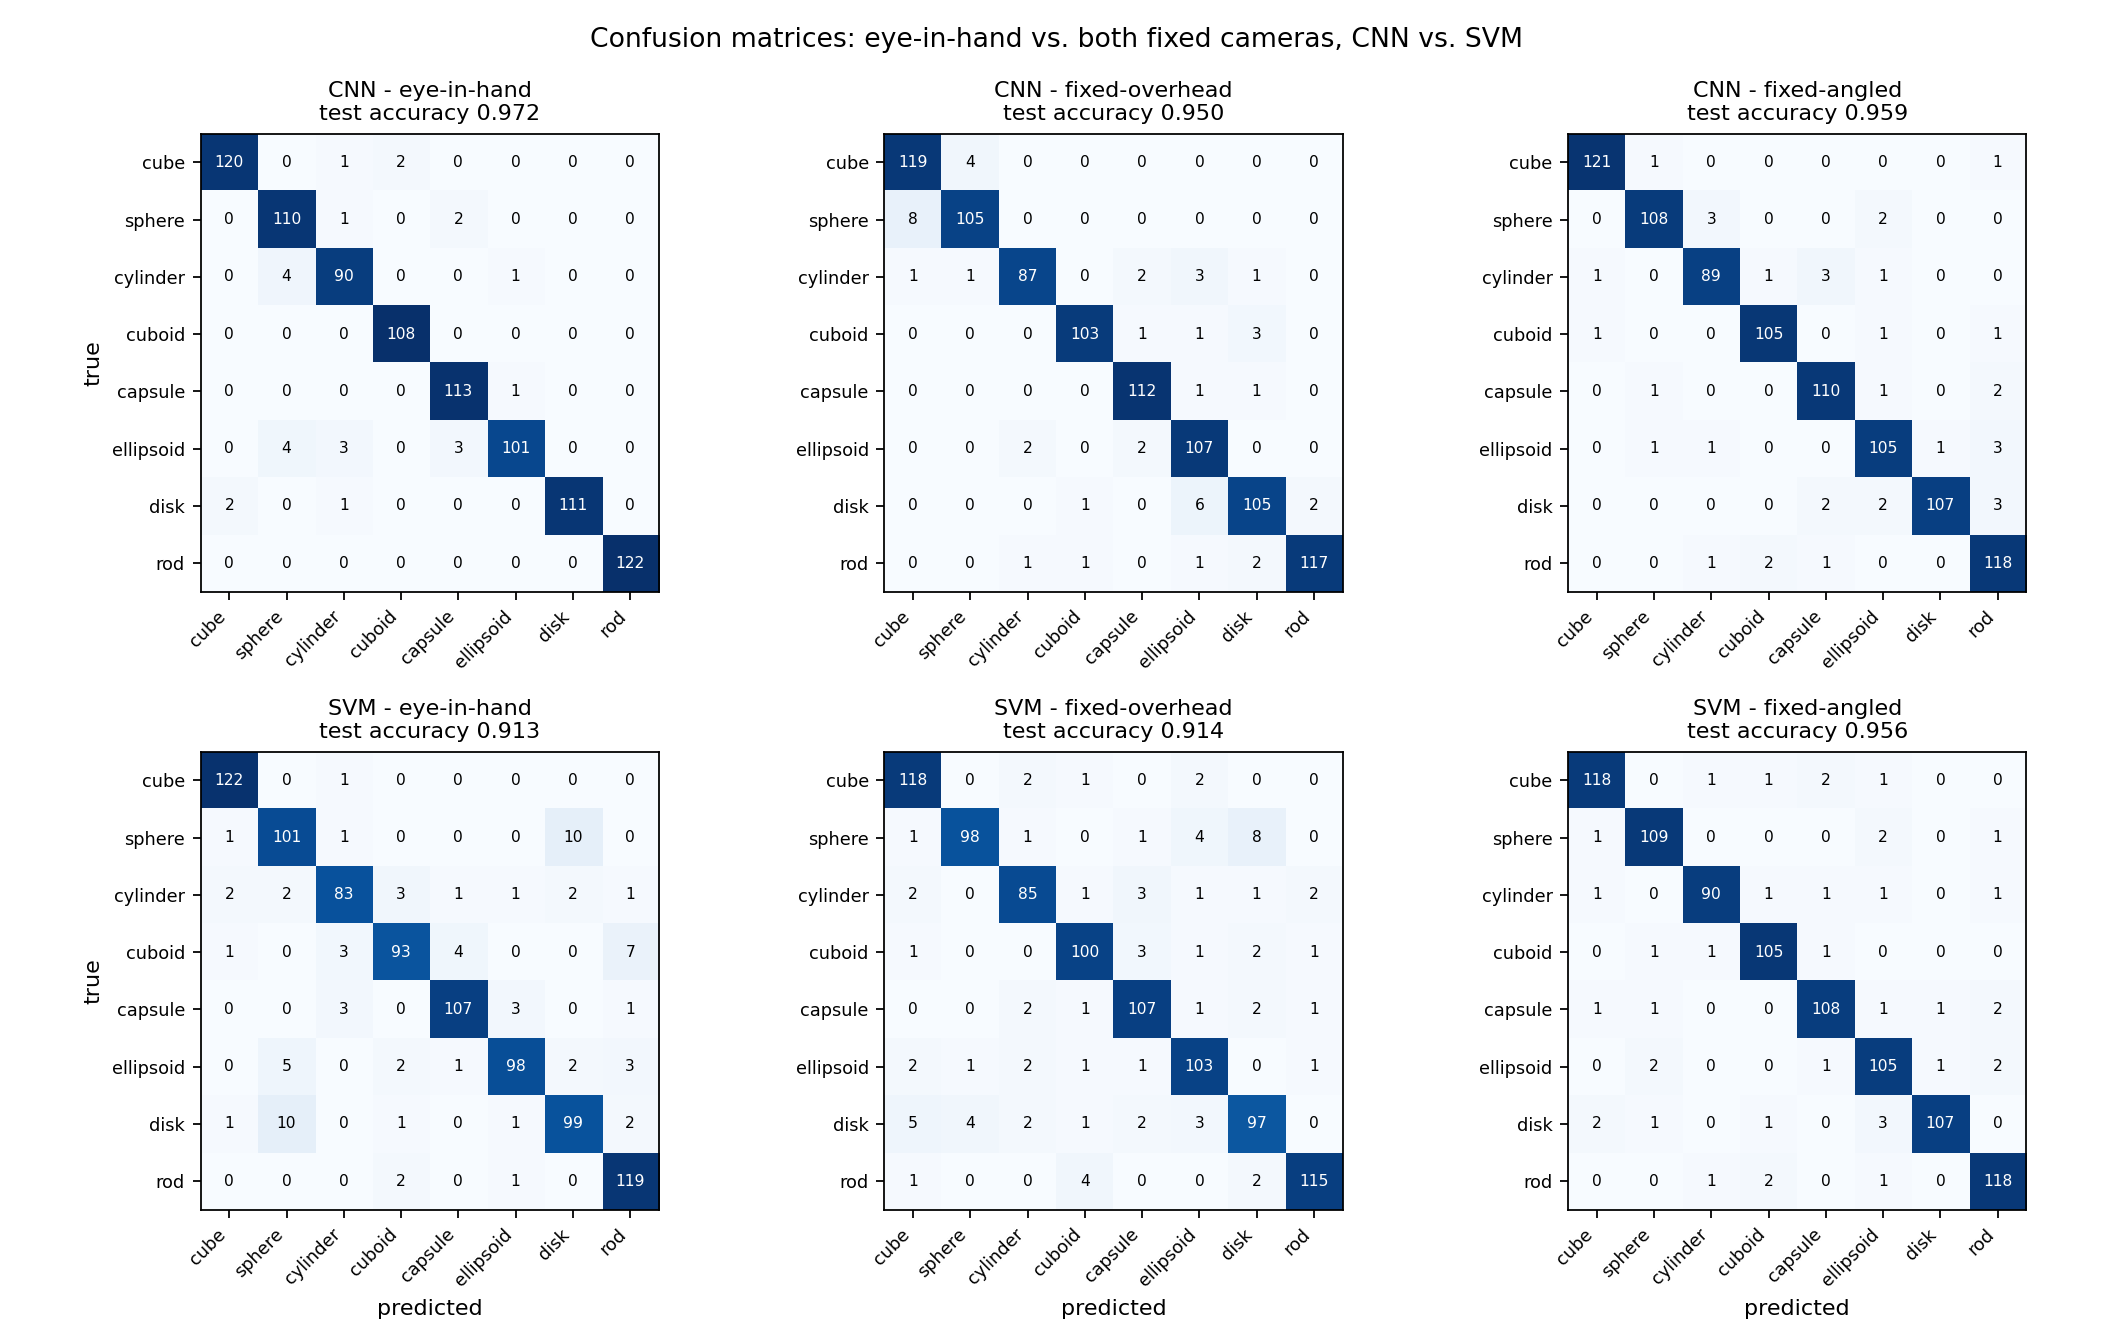
\includegraphics[width=0.85\linewidth]{figures/confusion_matrix.png}

\caption{Row-true, column-predicted confusion matrices, raw counts, for all six combinations.}

\label{fig:confusion}

\end{figure*}



\subsection{Statistical Significance}

All three views share the identical held-out test frame indices (Section 4), which licenses a paired analysis for each fixed camera against eye-in-hand (src/significance.py) -- more powerful than comparing two independent accuracies, because it asks ``on the instances where the two views disagree, which one is usually right?'' rather than ``are these two numbers different?''

\begin{table*}[t]

\centering

\caption{Paired bootstrap confidence intervals and McNemar's exact test for each fixed camera against eye-in-hand.}

\label{tab:significance}

\small

\begin{tabular}{llccccc}

\toprule

Fixed camera & Model & Eye-in-hand acc. [95\% CI] & Fixed acc. [95\% CI] & Gap [95\% CI] & McNemar's $p$ \\

\midrule

Fixed-overhead & CNN & 0.9722 [0.9611, 0.9822] & 0.9500 [0.9356, 0.9644] & +0.0222 [+0.0044, +0.0389] & 0.017 \\

Fixed-overhead & SVM & 0.9133 [0.8956, 0.9311] & 0.9144 [0.8956, 0.9322] & -0.0011 [-0.0267, +0.0256] & 1.000 \\

Fixed-angled (45 degrees) & CNN & 0.9722 [0.9611, 0.9822] & 0.9589 [0.9456, 0.9711] & +0.0133 [-0.0033, +0.0300] & 0.141 \\

Fixed-angled (45 degrees) & SVM & 0.9133 [0.8956, 0.9311] & 0.9556 [0.9422, 0.9689] & -0.0422 [-0.0644, -0.0200] & 0.000 \\

\bottomrule

\end{tabular}

\end{table*}



\begin{figure}[t]

\centering

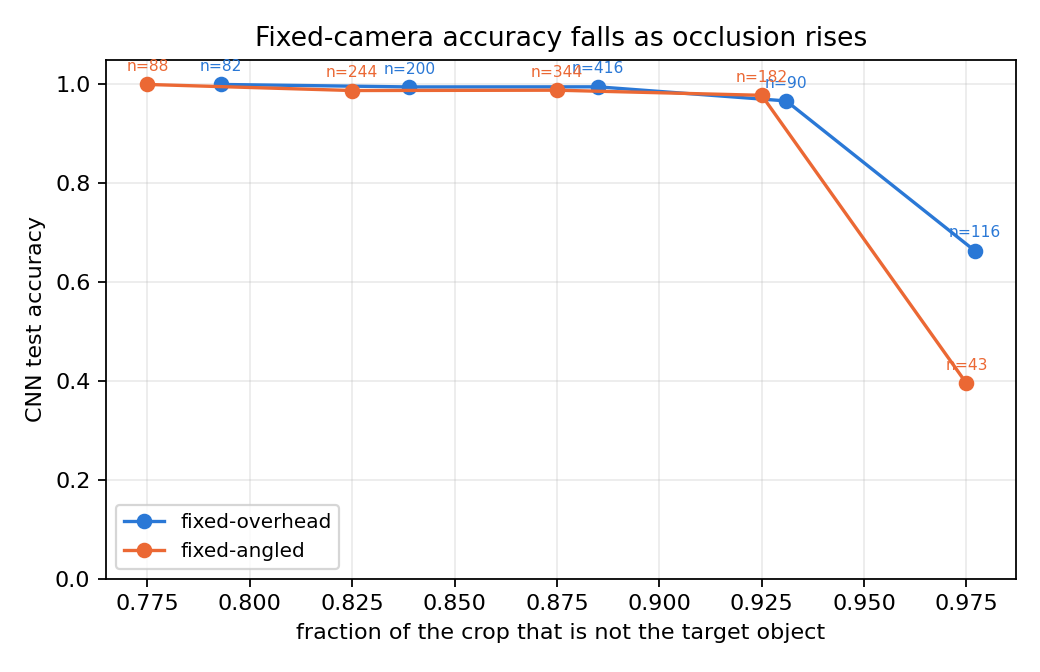
\includegraphics[width=\linewidth]{figures/occlusion_vs_accuracy.png}

\caption{Binning each fixed camera's CNN held-out predictions by occluded\_fraction shows accuracy falling as the crop fills with everything except the object, for both fixed cameras -- direct, per-sample evidence for the mechanism behind both accuracy gaps.}

\label{fig:occlusion}

\end{figure}



\begin{figure*}[t]

\centering

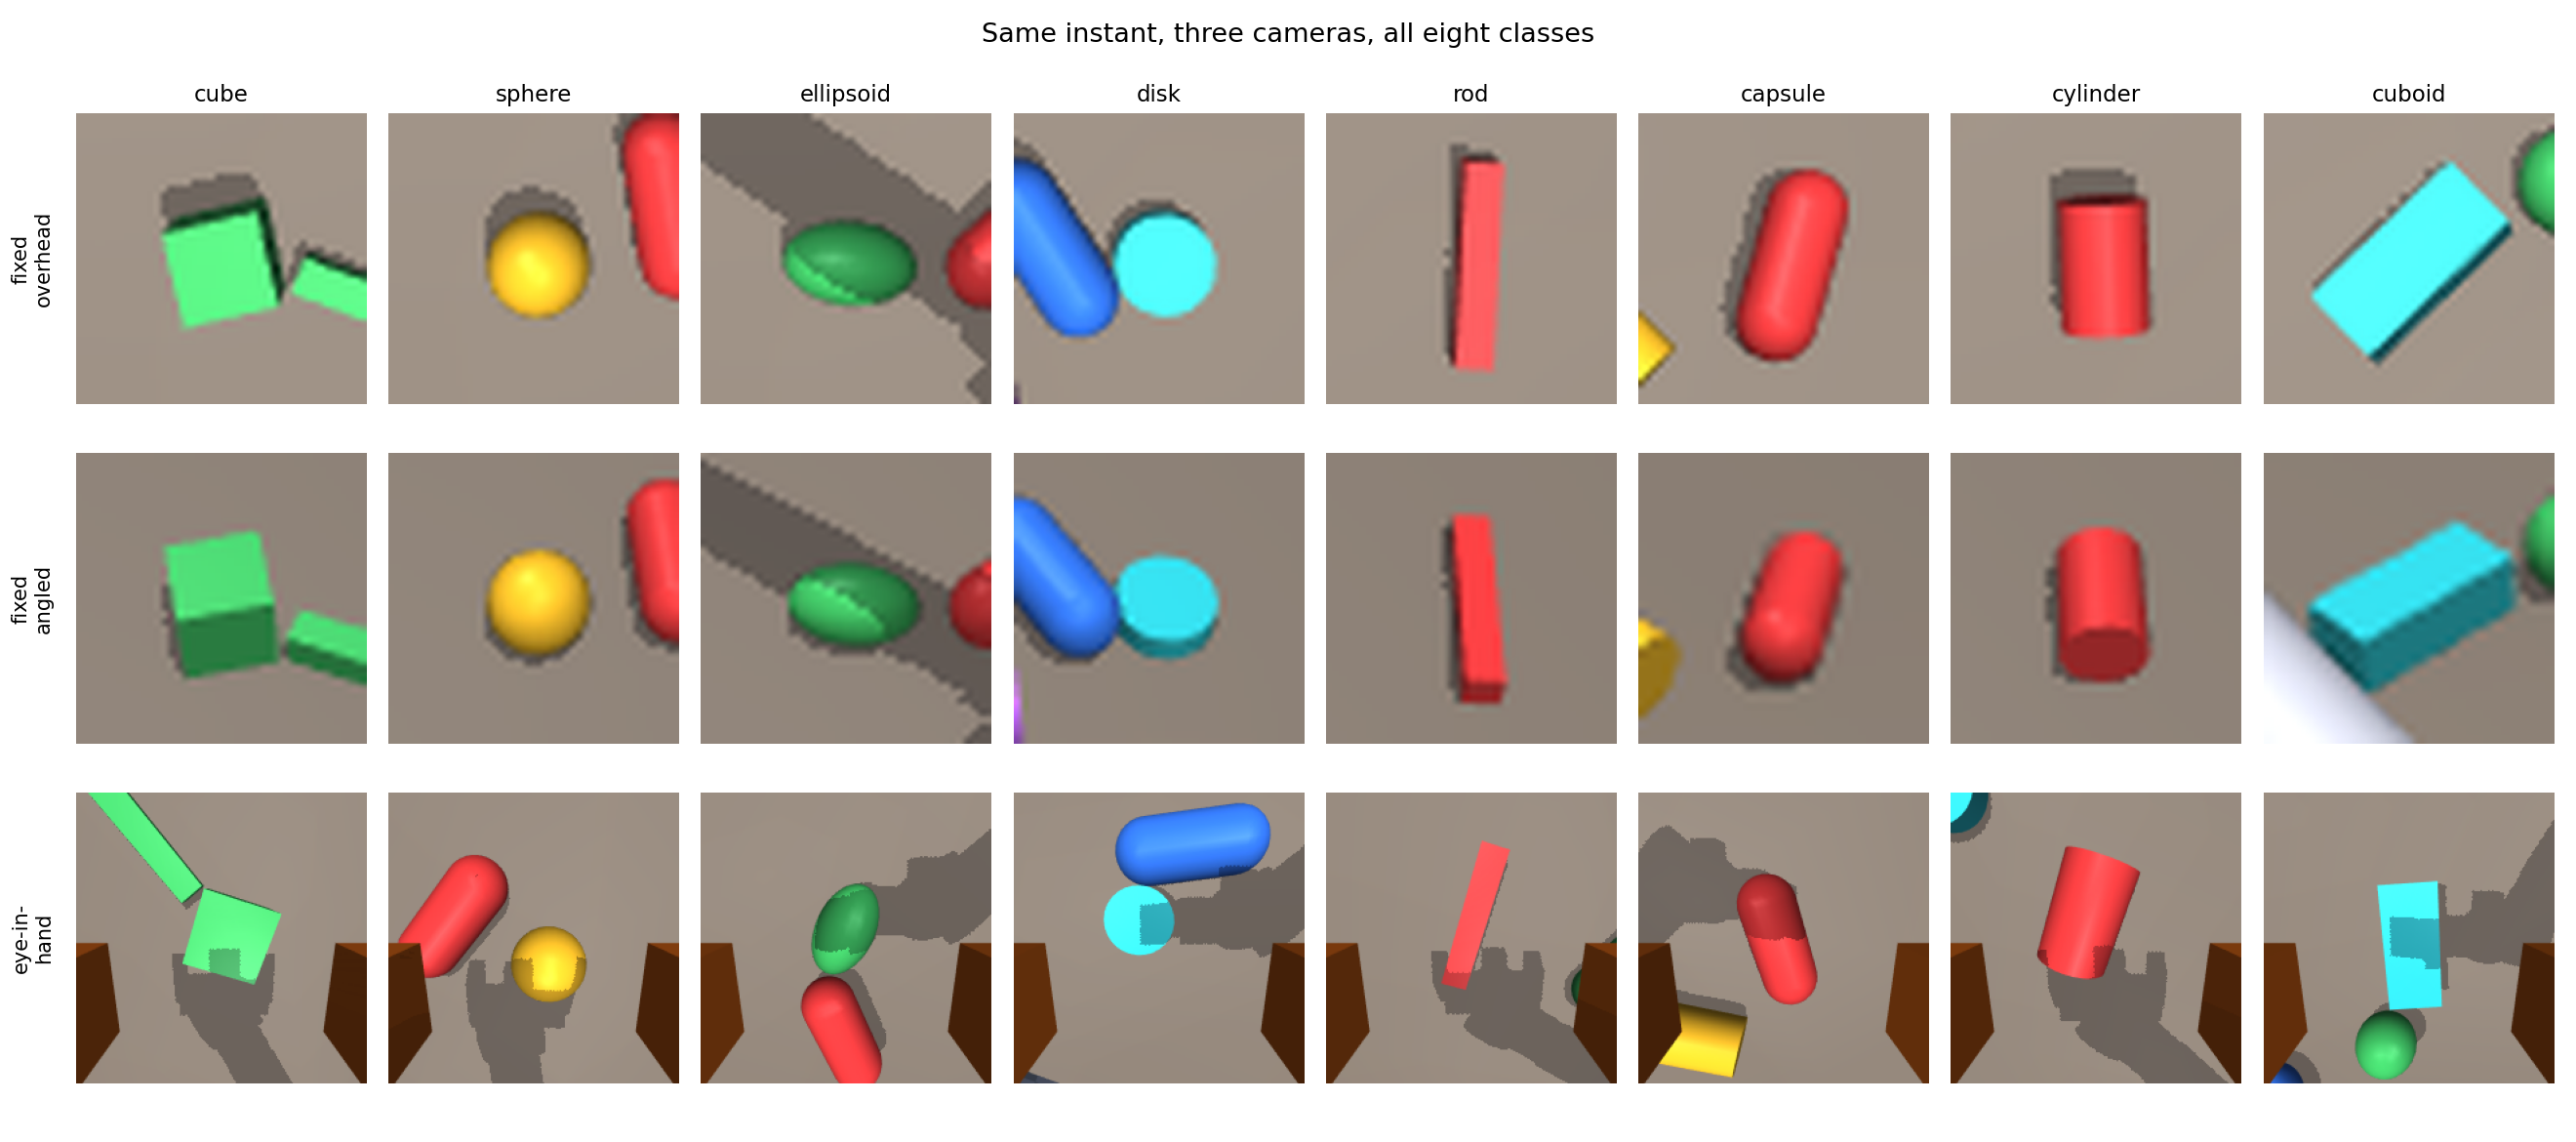
\includegraphics[width=0.9\linewidth]{figures/scale_comparison.png}

\caption{The same instant, all three cameras, all eight classes. The fixed-camera window is the same physical size regardless of class, so a sphere or ellipsoid fills far less of it than a rod or cuboid.}

\label{fig:scale}

\end{figure*}



\begin{figure*}[t]

\centering

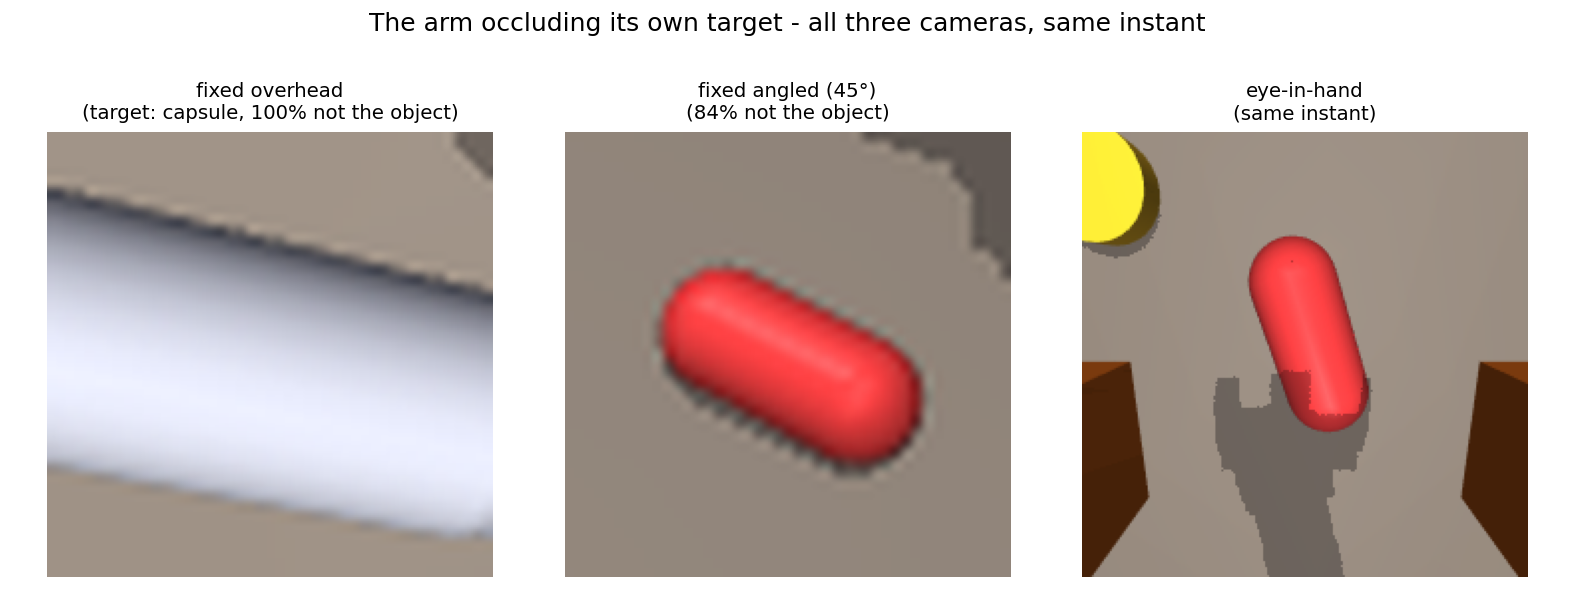
\includegraphics[width=0.9\linewidth]{figures/occlusion_demo.png}

\caption{The arm occluding its own target: at the instant the eye-in-hand camera frames this object cleanly, the fixed-overhead camera sees only the arm, while the fixed-angled camera, looking in from the side, still catches a partial view of the same object at the same instant.}

\label{fig:occlusion-demo}

\end{figure*}

\section{Discussion}

The main result is that eye-in-hand does not win outright. It is significantly more accurate than the fixed-overhead camera for the CNN (0.9722 vs. 0.9500 test accuracy, p=0.017), but the gap to the fixed-angled camera is smaller and not significant for the CNN (0.9722 vs. 0.9589, p=0.141). For the SVM, eye-in-hand and fixed-overhead are statistically tied (0.9133 vs. 0.9144, p=1.000), and eye-in-hand is significantly less accurate than the fixed-angled camera (0.9133 vs. 0.9556, p<0.001). We report all four comparisons rather than the two that happen to favour eye-in-hand, since a benchmark that only reports favourable comparisons is not a useful benchmark.

The comparison between the two fixed cameras explains most of this pattern. On the held-out test set, the fixed-overhead camera's crop is at least 95\% non-object on 14.0\% of frames (126 of 900); the fixed-angled camera reaches that level on 4.8\% (43 of 900). This matches the geometry: an arm reaching down toward an object sits between that object and a straight-down camera more often than it sits between the object and a camera looking in from the side. Accuracy on these near-fully-occluded frames is low for every camera and model (SVM: 56.3\% fixed-overhead, 32.6\% fixed-angled; CNN: 69.0\% fixed-overhead, 39.5\% fixed-angled), so a camera that lands in this bin more often loses more overall accuracy to it. This is consistent with mounting angle, not fixedness by itself, being the main source of the gap between the two fixed baselines.

The difference between the CNN and SVM results is most likely explained by how each model handles frames that are not near-fully-occluded. Both models reach a similar accuracy on those frames (CNN: 99.2\%-98.7\%; SVM: 97.2\%-98.7\%), so the SVM's lower overall accuracy comes largely from the occluded tail, which makes its total accuracy more sensitive to how often that tail occurs -- and hence more sensitive to which fixed camera is used. The CNN's higher accuracy on clear frames leaves less room for the occlusion-rate difference to change its overall accuracy, which is consistent with its smaller, non-significant gap against the fixed-angled camera.

The CNN outperforms the SVM on all three camera views (0.9722 vs. 0.9133 eye-in-hand; 0.9500 vs. 0.9144 fixed-overhead; 0.9589 vs. 0.9556 fixed-angled). The gap between the two model families is wider here than in a four-class version of this task run during development (90.0\% eye-in-hand SVM cross-validation accuracy at eight classes vs. 95.6\% at four classes), which is consistent with the eight-class taxonomy requiring shape discrimination that a bounding-box shortcut cannot provide. The SVM pipeline remains within a few points of the CNN on most cameras despite using a much simpler model with no learned features, which is relevant for a deployment where training or running a CNN is not practical.

\section{Limitations and Future Work}

\begin{enumerate}

  \item No domain randomisation. Lighting, table texture and camera intrinsics are fixed. A classifier trained on this data would almost certainly not transfer to a real camera. Randomising lighting direction and intensity, surface texture, and adding sensor noise and motion blur is the necessary next step before any sim-to-real claim.

  \item Geometric primitives, not real objects. Eight primitives -- four of them chosen specifically to be confusable with the other four -- prove the pipeline can measure a real difficulty gradient, not that it matches the task. Replacing them with scanned meshes of everyday objects is required before the classification problem is representative of a real picking workcell.

  \item Clutter in frame. Neighbouring objects appear at the edges of many frames in all three views. The labelled object is reliably centred, but frames are not clean single-object crops.

  \item Both fixed baselines are given the object's location for free. Their crops are centred on the target's known 3-D position; a real fixed-camera system would need its own detector or localiser to find that region first, which is not modelled here. The reported gaps are therefore the classification-only cost of each fixed viewpoint -- the true end-to-end cost, including detection failures under occlusion, is at least as large.

  \item The SVM's segmentation is a scene-specific shortcut, and an imperfect one. Isolating the silhouette by HSV-saturation thresholding works because objects are saturated and most of the scene is grey by construction -- except the claw's orange accent trim, which is also saturated, occasionally causing the largest saturated contour to be a finger rather than the object. This segmentation also would not survive a cluttered real background with its own saturated colours.

  \item Sample size. With one held-out test set per camera, not every accuracy gap in Table III reaches conventional statistical significance under a conservative paired test. A larger-scale replication, or an aggregated analysis across multiple random seeds, would sharpen these estimates rather than relying on a single test set per camera.

  \item Only one angle tested for the angled baseline. 45 degrees is one point on a continuum between straight-down and eye-level; whether occlusion and accuracy vary monotonically with mounting angle, or 45 degrees happens to sit at a particularly favourable or unfavourable point, is not established here.

  \item Grasping is open-loop. The claw closes to a width computed from ground-truth object geometry, which a real system would not have.

  \item Rigid-body contact only. Objects are rigid primitives with idealised friction. No deformables, no slip modelling.

\end{enumerate}

\section{Conclusion}

We built a simulated testbed that pairs an eye-in-hand camera with two independent fixed-camera baselines -- straight-overhead and 45-degree-angled -- observing the same manipulation task at the same instant over an eight-class taxonomy designed to resist a bounding-box shortcut, and used it to measure, rather than assume, the accuracy cost of the conventional fixed-camera design and whether that cost depends on mounting angle. The eye-in-hand camera does not win against both fixed baselines for both classifier families: it is significantly more accurate than the fixed-overhead camera with the CNN, roughly tied with the fixed-overhead camera with the SVM, and significantly less accurate than the fixed-angled camera with the SVM. A per-sample occlusion metric traces this pattern to a measured cause rather than an assumed one: the fixed-angled camera reaches near-full occlusion on a much smaller share of frames than the fixed-overhead camera, and this occlusion-rate difference affects the SVM's total accuracy more than the CNN's, since the SVM already loses more accuracy on occluded frames. The overall conclusion is that mounting angle, not fixedness by itself, is the main source of the accuracy cost usually attributed to a fixed camera, and that eye-in-hand's advantage over a fixed camera should not be assumed without specifying which fixed camera and which classifier are being compared. Two data-integrity bugs found during development, one a direct side effect of fixing the other, are reported for the same reason: an honest benchmark reports what was found, not only what was favourable. The complete pipeline, from procedural scene generation through trained model weights, is released so the benchmark can be extended, replicated at larger scale, tested at additional mounting angles, or subjected to domain randomisation as a step toward a genuine sim-to-real claim.

\section*{Acknowledgments}

The author thanks the DES Pune University CSE department and DRDO for research support.


\bibliographystyle{IEEEtran}
\bibliography{references}

\end{document}
